\chapter{Results}
\label{chap:results}
% ================================================================
\section{Competition's Dataset}
\label{section:competitions-dataset}
The user was shown a 6x6 matrix containing A..Z, 1..9 and \_ as shown in Chapter \ref{chap:approach}, Figure \ref{fig:p300-speller}. Each row and column was intensified once in a random sequence resulting in 12 intensifications in total. Each trial (12 intensification) was repeated 15 times which results in 180 total intensification per epoch. Each intensification lasts for 100ms followed by 75ms without any intensifications and so on. The above information are according to the description provided by competition 3 dataset 2.\par
% ----------------------------------------------------------------
Each subject (A and B) has 85 epoch (character) as train dataset and 100 epoch as test dataset. Figure \ref{fig:subject-A-p300} and Figure \ref{fig:subject-B-p300} shows the average of \ac{p300} plot for the 2 intensifications (row and column) that has the chosen character versus the 10 intensifications that does not contain the character.\par
\begin{figure}
    \centering
    \subfloat[
        Subject A \ac{p300} plot on train dataset on channel Cz.
        \label{subfig:subject-A-p300-train}
        ]{
            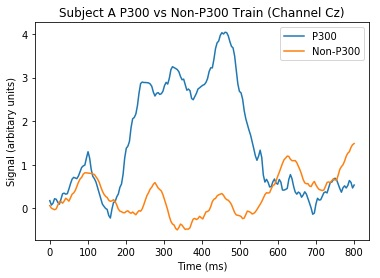
\includegraphics[width=\subFigureWidth]{images/results/subject_A_p300_train.jpg}
        }
    \hfill
    \subfloat[
        Subject A \ac{p300} plot on test dataset on channel Cz.
        \label{subfig:subject-A-p300-test}
        ]{
            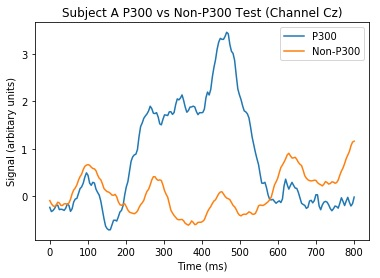
\includegraphics[width=\subFigureWidth]{images/results/subject_A_p300_test.jpg}
        }
    \caption{\ac{p300} plot of subject A.}
    \label{fig:subject-A-p300}
\end{figure}
\begin{figure}
    \centering
    \subfloat[
        Subject B \ac{p300} plot on train dataset on channel Cz.
        \label{subfig:subject-B-p300-train}
        ]{
            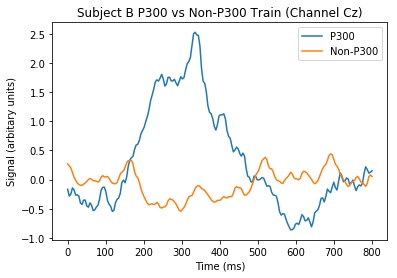
\includegraphics[width=\subFigureWidth]{images/results/subject_B_p300_train.jpg}
        }
    \hfill
    \subfloat[
        Subject B \ac{p300} plot on test dataset on channel Cz.
        \label{subfig:subject-B-p300-test}
        ]{
            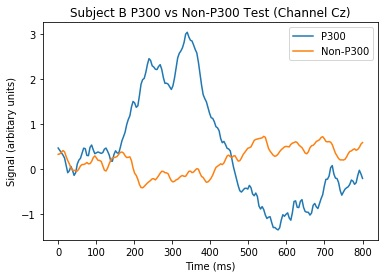
\includegraphics[width=\subFigureWidth]{images/results/subject_B_p300_test.jpg}
        }
    \caption{\ac{p300} plot of subject B.}
    \label{fig:subject-B-p300}
\end{figure}
% ----------------------------------------------------------------
Table \ref{tab:subject-A-B-char-reco} shows the character recognition analysis for subjects A and B according to the proposed channels mentioned in Sub-Section \ref{subsection:channel-selection}.\par
\begin{table}
    \centering
    \begin{tabular}{ c | c | c | c | c | c || c}
        \hline
        \textbf{Classifier} & \textbf{Channels} & \textbf{Window} & \textbf{Filters} & \textbf{A} & \textbf{B} & \textbf{Average} \\
        \hline\hline
        \multirow{8}{*}{\textbf{LDA}} & 8 & $0 \to 800ms$ & - & $73$ & $81$ & $77\pm4$\%\\
        {} & 8 & $0 \to 800ms$ & CarMaZsD & $79$ & $90$ & $84.5\pm5.5$\%\\
        
        {} & 8 & $200 \to 600ms$ & - & $71$ & $85$ & $78\pm7$\%\\
        {} & 8 & $200 \to 600ms$ & CarMaZsD & $65$ & $78$ & $71.5\pm6.5$\%\\
        
        {} & 64 & $0 \to 800ms$ & - & $81$ & $85$ & $83\pm2$\%\\
        {} & 64 & $0 \to 800ms$ & CarMaZsD & $89$ & $84$ & $86.5\pm2.5$\%\\
        
        {} & 64 & $200 \to 600ms$ & - & $86$ & $82$ & $84\pm2$\%\\
        {} & 64 & $200 \to 600ms$ & CarMaZsD & $82$ & $78$ & $80\pm2$\%\\
        \hline
    \end{tabular}
    \caption{Subject A and B character recognition rate.}
    \label{tab:subject-A-B-char-reco}
\end{table}
% ----------------------------------------------------------------
\clearpage
% ================================================================


\section{Recorded Dataset}
The same paradigm was applied as in Section \ref{section:competitions-dataset} same matrix, 12 intensifications, 15 repetitions, 100 ms for intensification and 75ms no intensification.\par
% ----------------------------------------------------------------
However, Each Subject (C and D) has 57 epoch as train dataset and 15 epoch as test dataset. Figure \ref{fig:subject-C-p300} and Figure \ref{fig:subject-D-p300} shows the average of \ac{p300} plot all 72 epochs.\par
\begin{figure}[!ht]
    \centering
    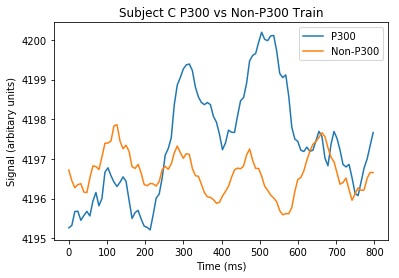
\includegraphics[width=\figureWidth]{images/results/subject_C_p300.jpg}
    \caption{Subject C \ac{p300} plot.}
    \label{fig:subject-C-p300}
\end{figure}
\begin{figure}[!ht]
    \centering
    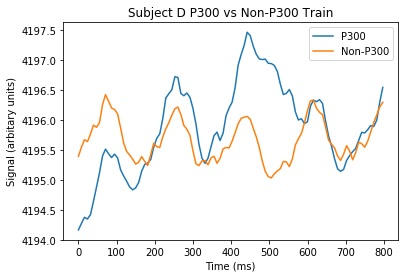
\includegraphics[width=\figureWidth]{images/results/subject_D_p300.jpg}
    \caption{Subject D \ac{p300} plot.}
    \label{fig:subject-D-p300}
\end{figure}
\clearpage
% ----------------------------------------------------------------

Table \ref{tab:subject-C-D-char-reco} shows the character recognition analysis for subjects C and D using the 14 channels of EMOTIV EPOCH+ Headset (Figure \ref{fig:emotiv-14-channels}).\par
\begin{table}[!ht]
    \centering
    \begin{tabular}{ c | c | c | c | c | c || c}
        \hline
        \textbf{Classifier} & \textbf{Channels} & \textbf{Window} & \textbf{Filters} & \textbf{A} & \textbf{B} & \textbf{Average} \\
        \hline\hline
        \multirow{4}{*}{\textbf{LDA}} & 14 & $0 \to 800ms$ & - & $53.36$ & $53.36$ & $53.36$\%\\
        {} & 14 & $0 \to 800ms$ & CarMaZsD & $86.67$ & $60$ & $73.33\pm13.33$\%\\
        {} & 14 & $200 \to 600ms$ & - & $46.67$ & $46.67$ & $46.67$\%\\
        {} & 14 & $200 \to 600ms$ & CarMaZsD & $46.67$ & $46.67$ & $46.67$\%\\
        \hline
    \end{tabular}
    \caption{Subject C and D character recognition rate.}
    \label{tab:subject-C-D-char-reco}
\end{table}
% ----------------------------------------------------------------
\clearpage
% ================================================================